\documentclass{beamer}

\usepackage{listings}
\usepackage{graphicx}
\usepackage{eiffel}

\newtheorem{purpose}{Purpose}

\lstset{language=OOSC2Eiffel, numbers=none}

\usetheme{SEChair}

\newcommand{\skipp}[0]{\vskip 0.5cm}
\newcommand{\skippause}[0]{\skipp \pause}

\title{SCOOP performance and implementation}

\author{Scott West}
\institute{ETH Z\"{u}rich}

\begin{document}
\maketitle

\begin{frame}
  \frametitle{Examining SCOOP performance}
  
  Since the research retreat:
  \begin{itemize}[<+->]
  \item Added the missing benchmarks that were discussed
  \item Added 2 more languages: Scala (Akka) actors and Java (mutex/condition variables)
  \item Started to investigate SCOOP performance and solutions
  \end{itemize}
\end{frame}


\begin{frame}
  \frametitle{Benchmark Overview}

  \begin{description}
  \item[condition] two groups of threads, each increments a shared variable when it is odd/even.
  \item[mutex] multiple threads contend for a critical section.
  \item[no share] threads do not share memory or coordinate, perform a computationally bound task.
  \item[prodcons] multiple producers and consumers work on a single queue.
  \item[share] multiple threads all threads share memory, but do not guard access to it (if possible)
  \end{description}
\end{frame}


\begin{frame}
  \frametitle{Benchmark results}
  \begin{center}
    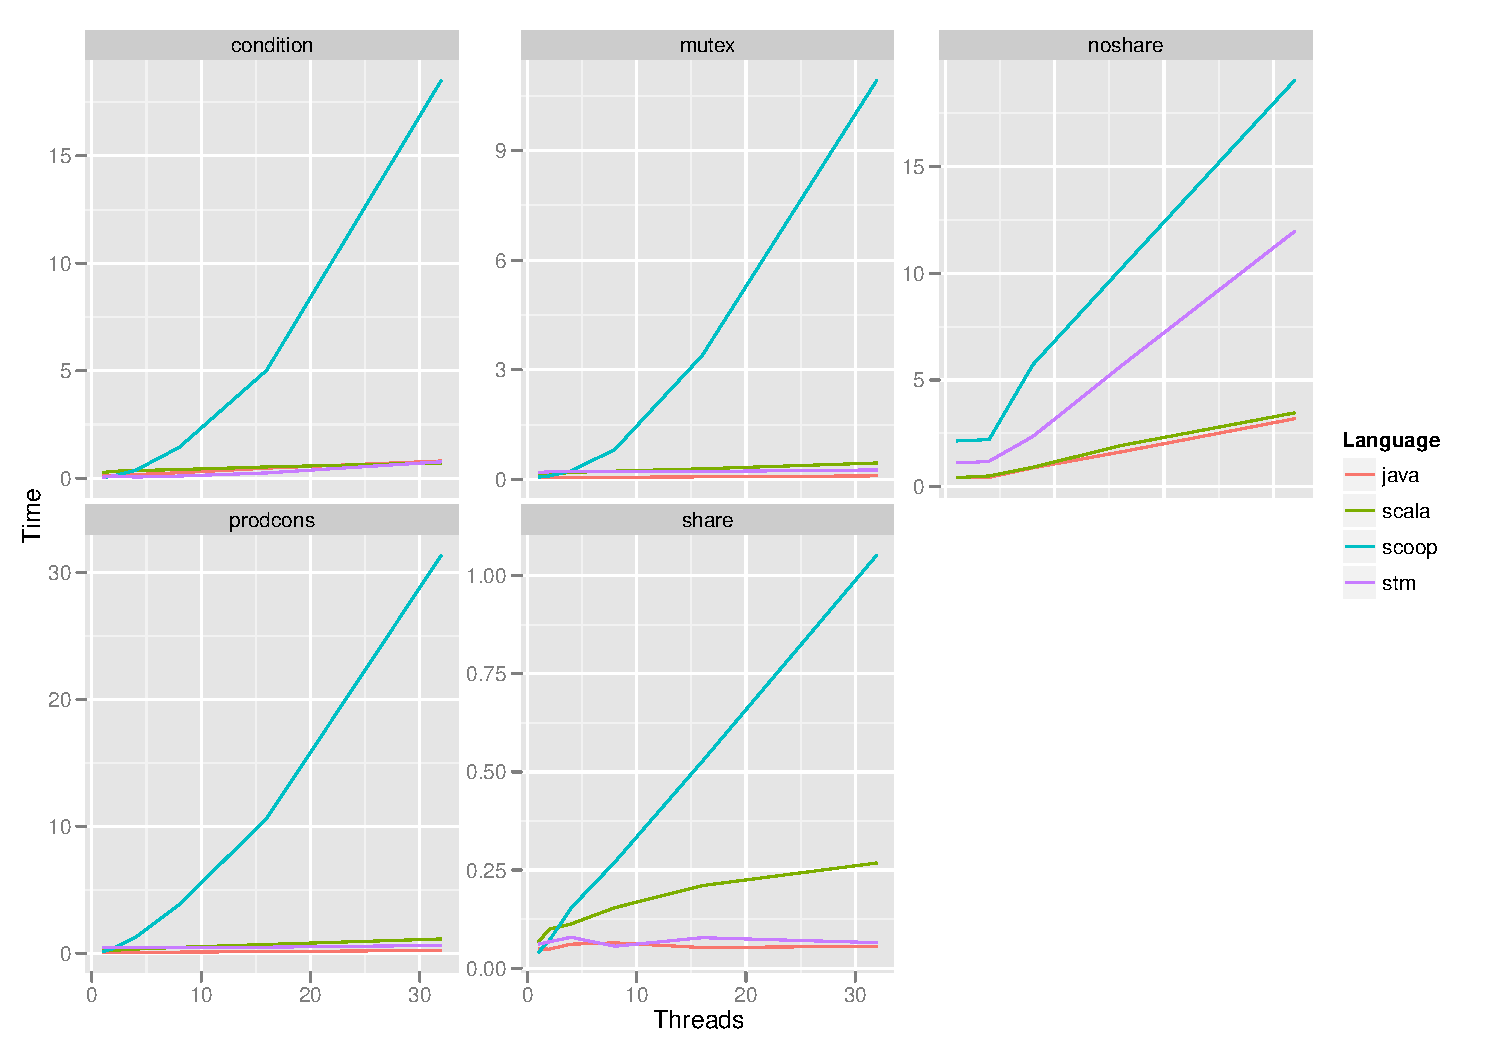
\includegraphics[width=4.5in]{time-facet-old}
  \end{center}
\end{frame}


\begin{frame}
  \frametitle{Next steps}
  Theme from last time: measure then cut.
  \begin{itemize}[<+->]
  \item SCOOP currently slows down superlinearly in the amount of work :(
  \item How do we find what we should cut? 
  \item Profiling and code inspection.
  \end{itemize}
\end{frame}

\begin{frame}
  \frametitle{SCOOP runtime: aimed at speed}
  
  \begin{itemize}
  \item Lots of atomic operations (compare and swap, atomic increment, etc.)
  \item Implemented records using arrays and offset indices to 
    avoid the object overhead.
  \item Avoids synchronization primitives (locks, semaphores).
  \end{itemize}  
\end{frame}

\begin{frame}[fragile]
  \frametitle{Resource acquisition}
  
  \begin{minipage}[c]{0.45\linewidth}
  \begin{lstlisting}
from
  acquired := False
until 
  acquired
loop
  old_val :=
    cas (resrc, free, this)
  if old_val = free then
    acquired := True
  else
    yield
  end
end
  \end{lstlisting}
\end{minipage}
\begin{minipage}[c]{0.45\linewidth}
  \begin{itemize}[<+->]
  \item This code avoids a mutex!
  \item Mutexes are slow because they may trigger context switch...
  \item ... but \emph{yield} also triggers a context switch.
  \item This code is basically a mutex but never sleeps and
    eats a core (it spins until it acquires the resource).
  \item Replacing it with a traditional mutex helps.
  \end{itemize}
\end{minipage}
\end{frame}

\begin{frame}
  \frametitle{Moving forward}

  \begin{itemize}[<+->]
  \item I started to rewrite the slow parts as best I could;
    these did lead to some improvements.
  \item However the changes are untestable: the code currently
    deadlocks and has some other bugs so
    I have no way to figure out if it's more or less broken 
    after my changes.
  \item Develop a ``laboratory'' where I can try out ideas: 
    proof-of-concept in C++.
  \end{itemize}
\end{frame}

\begin{frame}
  \frametitle{SCOOP implementation model}
  
  A SCOOP processor is basically a work-queue which
  other processors have exclusive access to.
  \begin{center}
    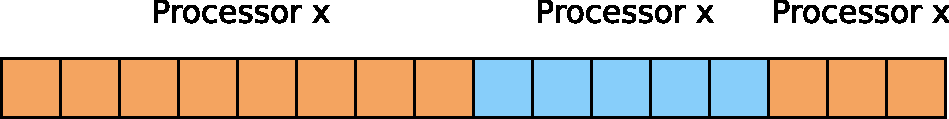
\includegraphics[width=3in]{queue-naive}
  \end{center}

  \pause
  Na\"ive implementation STL queue wrapped in a monitor: 404s

  \pause
  Non-blocking TBB queue: 180s

  \pause
  Blocking TBB queue: 108s

  \pause
  \vskip 1cm
  Is this any faster than what we have now?
  \pause

  Sort of, EiffelStudio 7.1: 33s but EiffelStudio 7.2: 155s.
\end{frame}

\begin{frame}
  \frametitle{SCOOP implementation model 2}
  
  Lock contention can be reduced if there is no
  memory to contend over:
  use a queue of queues

  \begin{center}
    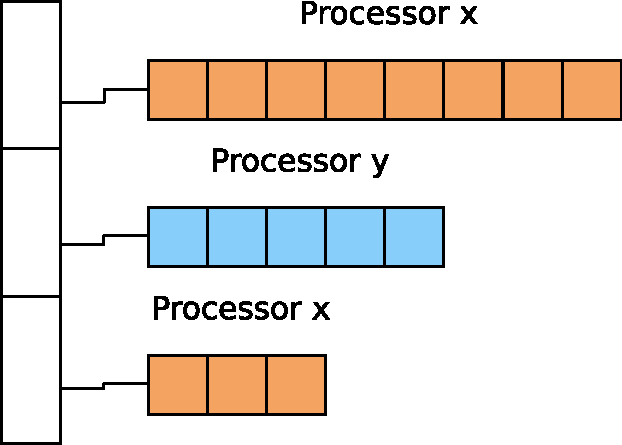
\includegraphics[width=2in]{queue-of-queues}
  \end{center}
  \pause
  Queue of queues: 15s.

  \pause
  With limited dequeue spinning: 3.7s

  \pause
  Don't use the queue for ``second'' queries: 2.0s
\end{frame}

\begin{frame}
  \frametitle{Putting them all together}

  \begin{center}
  \begin{tabular}{r|r}
    Approach &  Time  \\ \hline
    Blocking (STL wrapper)   &  404s \\
    TBB Non-blocking (sleep) &  180s \\
    ES 7.2                   &  155s \\
    TBB Blocking             &  108s \\
    ES 7.1                   &   33s \\
    Queue of queues          &   15s \\
    QoQ + Spinning           &  3.7s \\
    QoQ + Local queries      &  2.0s \\
  \end{tabular}
  \end{center}
\end{frame}

\begin{frame}
  \frametitle{EiffelStudio 7.1 vs. proof of concept}
  \begin{center}
    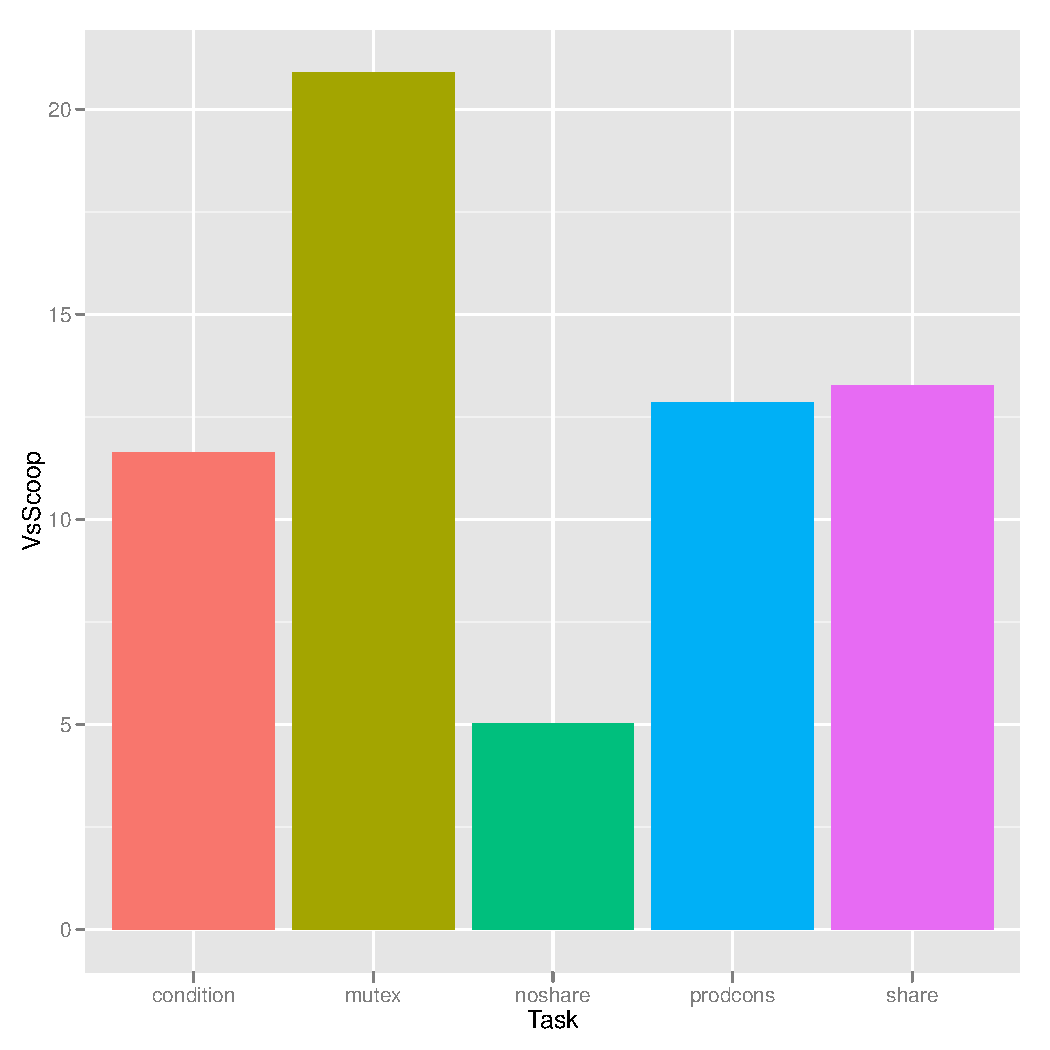
\includegraphics[width=3.2in]{share-bar}
  \end{center}
\end{frame}

\begin{frame}
  \frametitle{New benchmark results}
  \begin{center}
    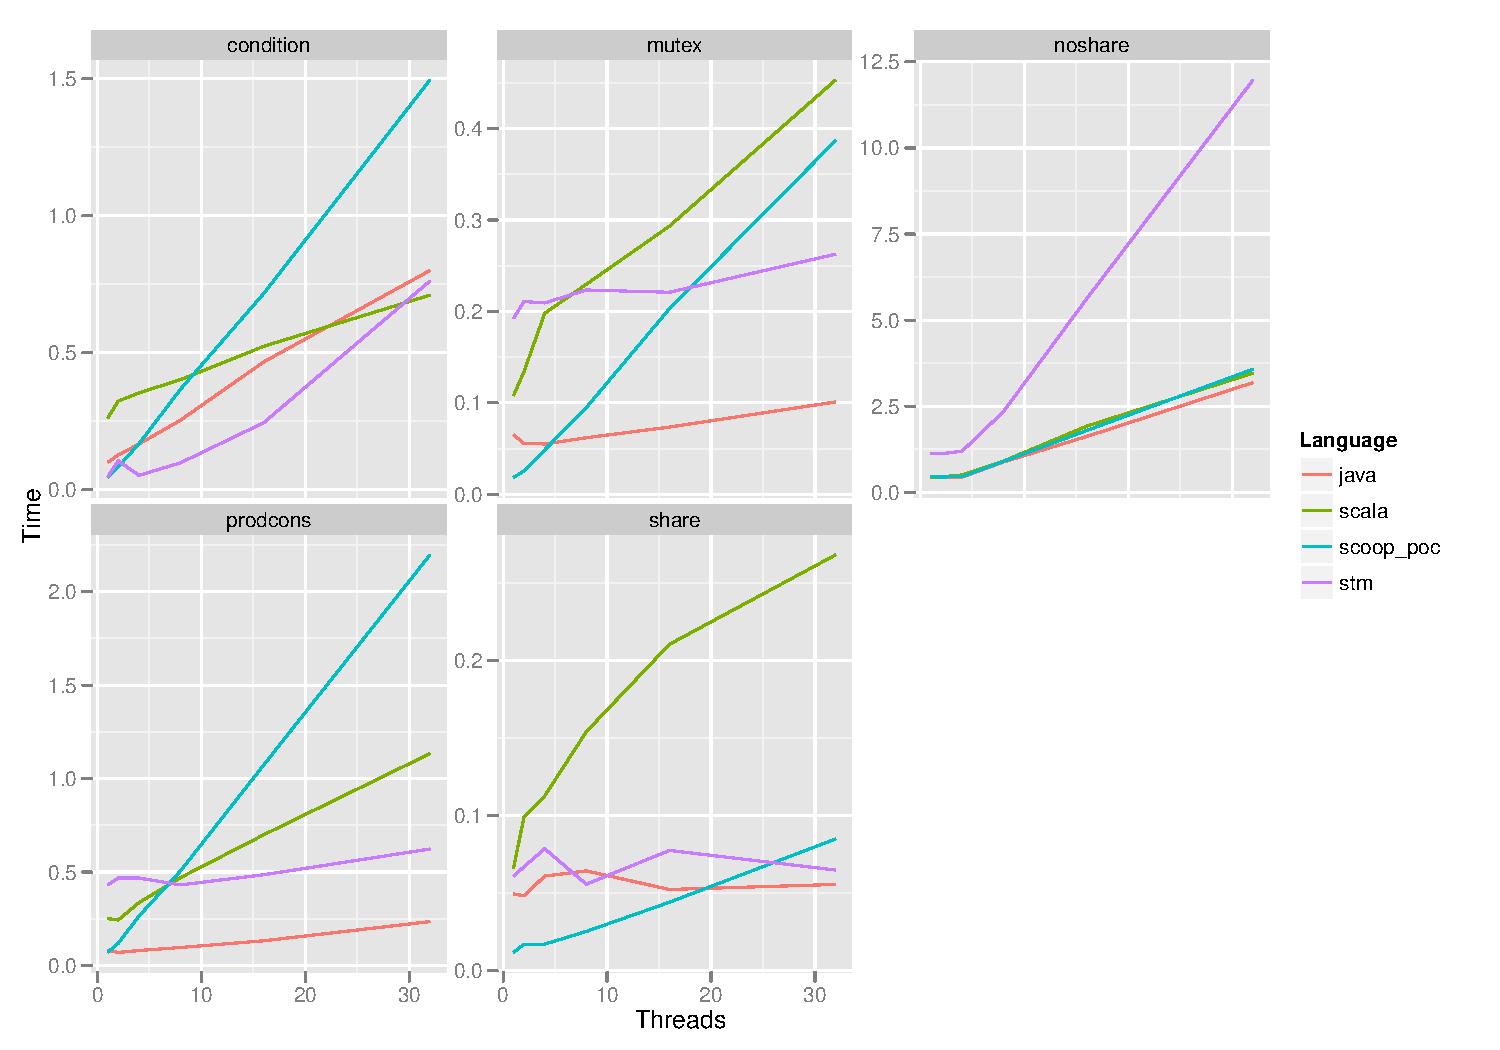
\includegraphics[width=4.5in]{time-facet-new}
  \end{center}
\end{frame}

\begin{frame}
  \frametitle{Implementation comments}

  \begin{itemize}
  \item The processor ``runtime'' is small: about 150 lines of C++.
  \item Seems to be the right target abstraction; almost no usage of
    explicit synchronization.
  \item Only one dependency, TBB.
  \item Probably still some room to fine tune, 
    i.e.\ use specialized queues where possible, like single-producer/consumer queues.
  \end{itemize}
\end{frame}


% \begin{frame}
%   \frametitle{Concurrency v. Parallelism}
%   \begin{definition}[Parallelism]
%     A program doing more than one thing at a time to compute a result faster.
%     The result is deterministic.
%   \end{definition}

%   \begin{definition}[Concurrency]
%     A program with multiple threads of control that which 
%     interleave in a non-deterministic way.
%   \end{definition}

%   They are not exclusive: concurrency can be used to implement parallelism.
% \end{frame}

% \begin{frame}
%   \frametitle {Our task}
%   A performance benchmark should be a way to measure a relevant aspect
%   of execution properties.
%   \skippause
%   Parallelism benchmarks define a task that should have the same result
%   every time, and the result must arrive quickly!
%   \skippause
%   We aim to define a way to benchmark concurrent programs.
% \end{frame}

% \begin{frame}
%   \frametitle{What is a concurrent benchmark?}
%   Since a concurrent program executes nondeterministically,
%   benchmarking will concern profiling the performance characteristics
%   of various \emph{synchronization}, \emph{communication}, and \emph{coordination} 
%   tasks.
% \end{frame}

% \begin{frame}
%   \frametitle{Benchmark Overview}
%   We wish to examine \emph{scalability}: how does a benchmark react to 
%   increased contention/threads/problem size.

%   We will examine concurrent programs with multiple patterns:

%   \begin{description}
%   \item[no share] threads do not share memory or coordinate.
%   \item[1-N comm.] a single master thread dispatches work to multiple workers.
%   \item[M-N comm.] multiple master threads dispatch work
%   \item[mutex] multiple threads contend for a critical section with high contention.
%   \item[benign share] threads share memory, but do not have guarded access to it.
%   \end{description}
% \end{frame}

% \begin{frame}[fragile]
%   \frametitle{Noninterference}
%   \begin{purpose}
%     To test the cost of running multiple threads by the runtime system.
%   \end{purpose}

%   Some concurrency abstractions have non-trivial departures from
%   POSIX-like threads (such as green threads) and
%   this such a test would determine the effect of any such abstractions.
%   \skipp
%   This would take the shape of running some compute heavy task
%   in each thread. I,e.

%   \begin{lstlisting}
%     fib (30)
%   \end{lstlisting}

% \end{frame}

% \begin{frame}
%   \frametitle{1-N communication}
%   \begin{purpose}
%     To examine the cost of having multiple threads contending for a single event.
%   \end{purpose}
  
%   This test replicates a common design in server applications where a main thread
%   dispatches work to multiple reader threads.
%   \skipp
%   The test will have a single channel of communication where the master
%   dispatches integers to the workers.
%   The workers continually receive and discard the integers.
% \end{frame}

% \begin{frame}
%   \frametitle{M-N communication}
%   \begin{purpose}
%     To test the effect of multiple producers accessing a single consumption channel.
%   \end{purpose}

%   Similar to the previous test, but with multiple masters and workers at either end
%   of the work distribution.
% \end{frame}

% \begin{frame}
%   \frametitle{Mutex}
%   \begin{purpose}
%     To quantify the cost of gaining exclusive access to a critical section.
%   \end{purpose}

%   The critical section should be heavily contended as this is the case where
%   performance issues tend to arise.

%   The mutex operations may be noops (if a CS is not explicitly required),
%   but \emph{must} update some shared state in a simple way (ie, adding 1).
% \end{frame}

% \begin{frame}
%   \frametitle{Interfering}
%   \begin{purpose}
%     To examine the overhead of continually accessing a shared resource without
%     any extra protection not provided by the implementation.
%   \end{purpose}

%   Very often there are benign dataraces, this test quantifies the performance
%   cost of modifying shared memory without an explicit mutex protecting it.
% \end{frame}

% \begin{frame}
%   \frametitle{Preliminary results}

%   \begin{center}
%     \begin{tabular}[h]{l|l|l}
%       Benchmark    & STM (Haskell) & SCOOP \\ \hline
%       No share     &     --        &--     \\
%       1-N comm.    &       --      &  --   \\
%       M-N comm.    & 0.478 s       & 63.747 s \\
%       Mutex        & 0.067 s       & 24.235 s \\
%       Benign share &        --     &   --  \\
%     \end{tabular}
%   \end{center}
% \end{frame}

% \begin{frame}
%   \frametitle{Going further}
%   \begin{itemize}
%   \item Add more microbenchmarks, gathered from real situations.
%   \item Implement the benchmarks in various concurrency approaches,
%     with a focus on languages that focus on concurrency rather than
%     data parallelism.
%     \begin{itemize}
%       \item Candidates for other approaches: Erlang, Go, Ada, Clojure, F\#, D, Java, Scala, Orc...
%     \end{itemize}
%   \item Validation step: use them to predict performance of larger programs.
%   \end{itemize}
% \end{frame}

\end{document}
